%\documentclass[tikz]{standalone}

%\begin{document}

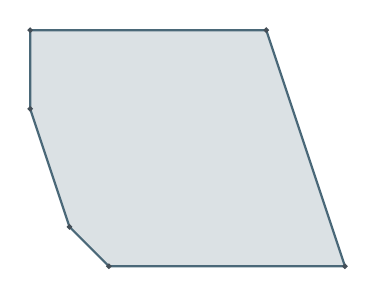
\begin{tikzpicture}%
	[scale=.010,
	edge/.style={color=cyan!40!black, thick},
	facet/.style={fill=cyan!40!black, fill opacity=0.2},
	vertex/.style={inner sep=0pt,circle,draw=cyan!25!black,fill=cyan!75!black,thick,anchor=base}]
%%
%% Drawing the facets
%%
\fill[facet] (-300.0, 300.0) -- (-300.0, 200.0) -- (-250.0, 50.0) -- (-200.0, 0.0) -- (100.0, 0.0) -- (0.0, 300.0) -- cycle {};
%%
%% Drawing edges in the front
%%
\draw[edge] (-300.0, 300.0) -- (-300.0, 200.0) -- (-250.0, 50.0) -- (-200.0, 0.0) -- (100.0, 0.0) -- (0.0, 300.0) -- cycle {};
%%
%% Drawing the vertices in the front
%%
\node[vertex] at (-300.0, 300.0) {};
\node[vertex] at (-300.0, 200.0) {};
\node[vertex] at (-250.0, 50.0) {};
\node[vertex] at (-200.0, 0.0) {};
\node[vertex] at (100.0, 0.0) {};
\node[vertex] at (0.0, 300.0) {};
%%
\end{tikzpicture}

%\end{document}